%----------------------------------------------------------------------------------------
%	INITIAL TEST.
%----------------------------------------------------------------------------------------
\subsection{Initial test}


\begin{figure}[H]
\centering
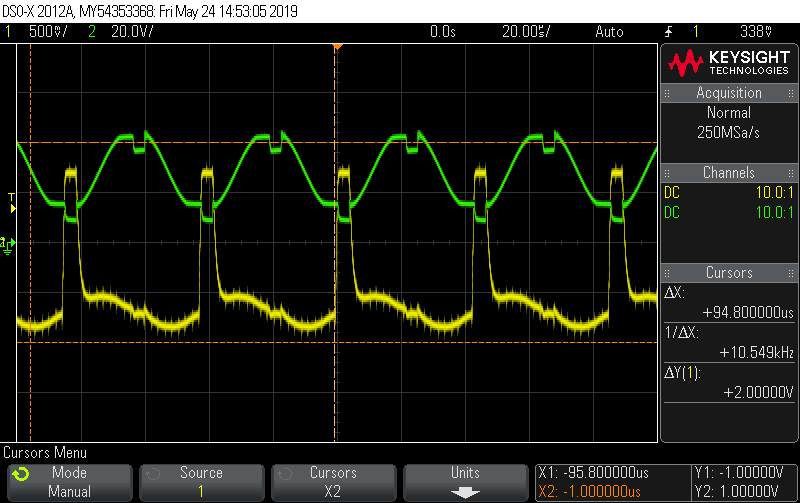
\includegraphics[width=.9\textwidth]{figures/scope_20.png}
\caption{High voltage output is connected. In yellow the input 'TP2' to the power switch is shown and in green the output 'TP1' of the switch, controlling the transformer. It can be seen that the transformer is in resonance.}
\label{fig:scope_20}
\end{figure}


We had an ugly signal, the high voltage output was 3176\,V


In order to get this output, we had to re-adjust the clock frequency of the oscillator 'CLK'.


The high voltage output voltage then increased to 3225\,V.

